\section{Latent-Space GMM Experiments \& Diagnostic Evidence}
\label{sec:p2_latent_gmm_results}

This section reports the empirical evaluation of Hybrid H1 (latent-space Gaussian mixture density scoring) built atop the Phase~2 Autoencoder bottleneck defined in Section~\ref{sec:p2_architecture} and analyzed theoretically in Section~\ref{sec:p2_hybrid_theory}. All models are trained strictly on legitimate training transactions ($170{,}524$ rows; $136{,}419$ train-sub and $34{,}105$ early-stop rows during model selection, refitted on all $170{,}524$ legitimate training rows for final evaluation), using Vani's frozen encoder interface \texttt{load\_autoencoder()} and \texttt{encode()} over the $d=31$ standardized \texttt{base} features.

\subsection{Configuration Selection: BIC vs.\ Validation PR-AUC}
\label{subsec:latentgmm_selection}

We evaluated a structured grid over covariance structures $\mathcal{C} = \{\mathrm{full}, \mathrm{tied}, \mathrm{diag}, \mathrm{spherical}\}$, component counts $K \in \{1, 2, 4, 8, 12, 16, 20, 24\}$, and covariance regularization $\varepsilon \in \{10^{-6}, 10^{-4}, 10^{-2}, 10^{-1}\}$ on latent representations $\mathbf{z} \in \mathbb{R}^{12}$ extracted from \texttt{ae\_best.pt} (undercomplete AE with hidden widths $[32, 16]$ and LeakyReLU bottleneck, Section~\ref{sec:p2_ae_results}). Table~\ref{tab:latentgmm_selection} contrasts unsupervised BIC selection \cite{schwarz1978estimating,akaike1974new} against supervised validation PR-AUC selection.

\begin{table}[!t]
\centering
\caption{Latent-GMM Configuration Selection Criteria on \texttt{ae\_best.pt} ($d_z = 12$)}
\label{tab:latentgmm_selection}
\begin{tabular}{lcccccr}
\toprule
Selection Rule & Cov. & $K$ & $\varepsilon$ & Params & Val BIC & Val PR-AUC \\
\midrule
Min Train-Legit BIC & full & 16 & $10^{-6}$ & 1,455 & 1,286,219 & 0.0520 \\
Min Val-Legit BIC   & full & 16 & $10^{-2}$ & 1,455 & 1,217,896 & 0.0575 \\
Max Val PR-AUC      & diag & 12 & $10^{-2}$ &   299 & 1,716,652 & \textbf{0.1510} \\
\bottomrule
\end{tabular}
\end{table}

Consistent with the density--anomaly mismatch analysis of Chandola et~al.~\cite{chandola2009anomaly} and Aggarwal~\cite{aggarwal2017outlier}, pure unsupervised BIC favors a high-capacity $\mathrm{full}$-covariance mixture ($K=16$, $1{,}455$ free parameters) that achieves lower held-out legitimate BIC ($1{,}217{,}896$ vs.\ $1{,}716{,}652$) but reaches only $0.0575$ validation PR-AUC ($0.5088$ Recall@0.5\%~FPR). Constraining covariance to $\mathrm{diag}$ with $K=12$ and $\varepsilon = 10^{-2}$ reduces the parameter count by $4.87\times$ (to $299$ parameters) while raising selection-split validation PR-AUC to $0.1510$ ($0.7193$ Recall@0.5\%~FPR), as illustrated in Fig.~\ref{fig:latentgmm_aic_bic}.

\begin{figure}[!t]
\centering
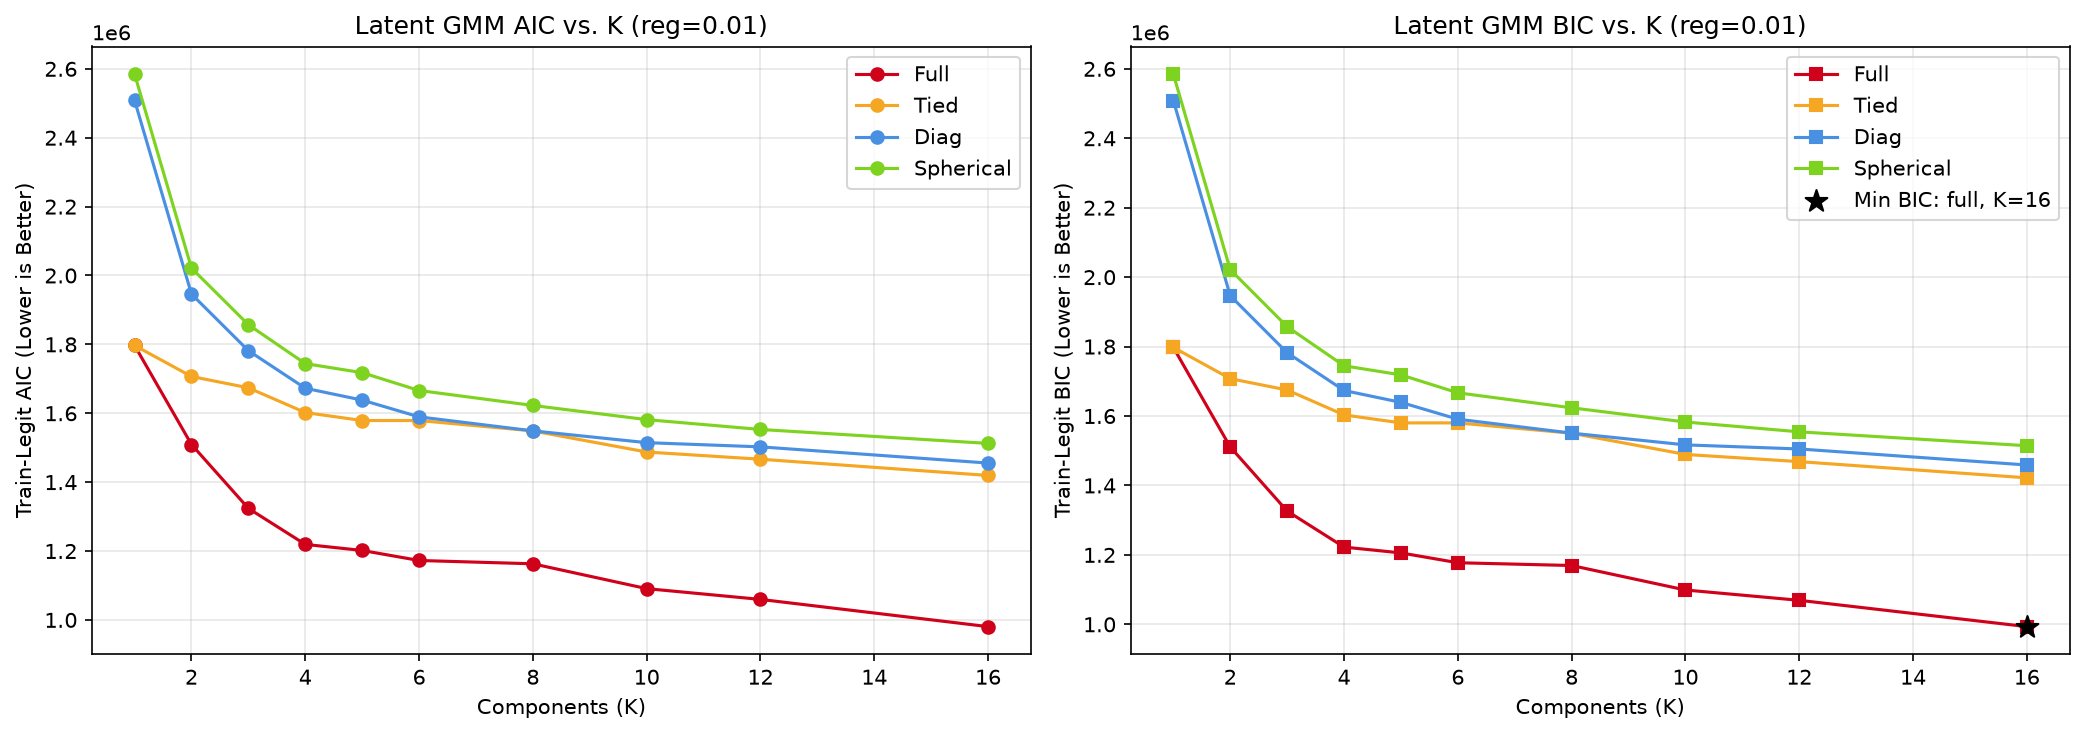
\includegraphics[width=\linewidth]{results/figures/latentgmm_aic_bic.png}
\caption{Latent-GMM grid search over component count $K$ and covariance structure on \texttt{ae\_best.pt} ($d_z=12$), contrasting unsupervised information criteria (AIC/BIC) with validation PR-AUC.}
\label{fig:latentgmm_aic_bic}
\end{figure}

\subsection{Final Hybrid H1 Performance and Parent Comparison}
\label{subsec:latentgmm_parents}

Refitting the validation-selected configuration ($\mathrm{diag}$, $K=12$, $\varepsilon=10^{-2}$) on all $170{,}524$ legitimate training transactions yields the frozen \texttt{hybrid\_latentgmm} scores. On the held-out test set ($75$ frauds), H1 attains PR-AUC $= 0.1724$ (95\% bootstrap CI $[0.1329, 0.2310]$), ROC-AUC $= 0.9398$, Recall@0.5\%~FPR $= 0.7467$ ($[0.6400, 0.8533]$), Recall@1.0\%~FPR $= 0.7867$, and Precision@$K=100$ $= 0.3000$ ($40.0\%$ fraud capture in the top $100$ alerts). On validation ($57$ frauds), H1 achieves PR-AUC $= 0.1159$, ROC-AUC $= 0.9302$, Recall@0.5\%~FPR $= 0.7018$, and Recall@1.0\%~FPR $= 0.7193$.

\begin{table}[!t]
\centering
\caption{Test-Set Comparison Against Phase~1 and Phase~2 Parent Models (95\% Paired Bootstrap CIs)}
\label{tab:latentgmm_parents}
\begin{tabular}{lcccc}
\toprule
Model & Val PR & Test PR-AUC [CI] & ROC-AUC & Rec@0.5\% [CI] \\
\midrule
Hybrid H1 (Latent GMM) & 0.1159 & 0.1724 [0.1329, 0.2310] & \textbf{0.9398} & 0.7467 [0.6400, 0.8533] \\
Phase~1 GMM (on disk)  & 0.1038 & 0.2679 [0.1843, 0.3800] & 0.9391 & 0.6667 [0.5467, 0.7600] \\
Phase~2 AE (\texttt{ae\_best}) & 0.2272 & 0.3574 [0.2618, 0.4848] & 0.9021 & 0.6800 [0.5733, 0.7733] \\
Phase~2 DAE (\texttt{ae\_dae}) & 0.2935 & 0.4818 [0.3707, 0.6166] & 0.9322 & \textbf{0.7733} [0.6667, 0.8667] \\
Phase~1 PCA            & 0.7066 & \textbf{0.7425} [0.6415, 0.8368] & 0.9303 & \textbf{0.7733} [0.6667, 0.8667] \\
\bottomrule
\end{tabular}
\end{table}

Table~\ref{tab:latentgmm_parents} reveals an instructive metric divergence. Paired bootstrap testing shows H1's test PR-AUC is significantly lower than all four parent baselines ($\Delta = -0.0955$ vs.\ Phase~1 GMM, $[-0.1923, -0.0185]$; $\Delta = -0.1849$ vs.\ AE, $[-0.2935, -0.0915]$; $\Delta = -0.3094$ vs.\ DAE, $[-0.4162, -0.2259]$; $\Delta = -0.5701$ vs.\ PCA, $[-0.6311, -0.4948]$). Yet at the operational $0.5\%$ FPR alert budget, H1 achieves the highest test ROC-AUC ($0.9398$) and improves test Recall@0.5\%~FPR by $+8.00$ percentage points over Phase~1 GMM ($0.7467$ vs.\ $0.6667$) and $+6.67$ points over its own encoder parent AE ($0.7467$ vs.\ $0.6800$). Fig.~\ref{fig:latentgmm_nll_dist} displays the separation between legitimate and fraud NLL distributions.

\begin{figure}[!t]
\centering
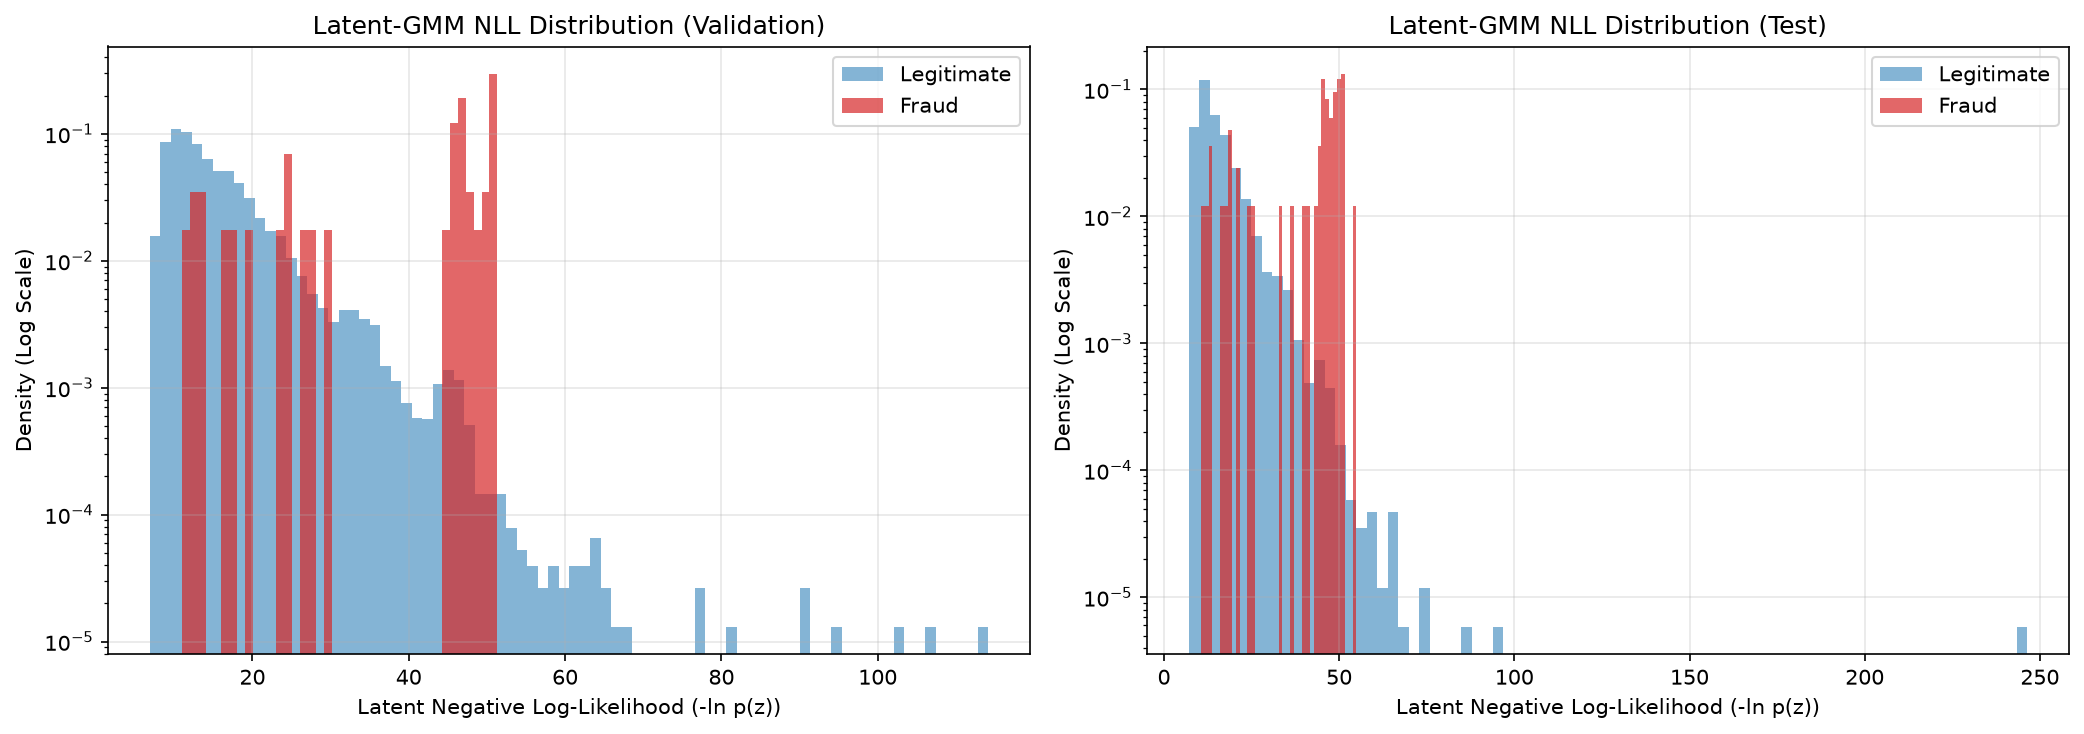
\includegraphics[width=\linewidth]{results/figures/latentgmm_nll_distribution.png}
\caption{Latent-GMM negative log-likelihood score distributions on validation and test splits, highlighting legitimate right-tail overlap alongside strong bulk fraud separation at the 0.5\% FPR operating threshold.}
\label{fig:latentgmm_nll_dist}
\end{figure}

\subsection{Numerical Conditioning, Seed Stability, and Latent Non-Gaussianity}
\label{subsec:latentgmm_diagnostics}

To explain both the stability gains and the PR-AUC shortfall, we conducted five diagnostic studies:

\paragraph{Parameter-Count Scaling ($d=30/31$ vs.\ $d_z=8/12$).}
Full-covariance mixture complexity scales quadratically as $M(K,d) = (K-1) + K d + \frac{1}{2} K d(d+1)$. At $K=12$ components, fitting a $\mathrm{full}$-covariance GMM in raw ambient space requires $5{,}951$ free parameters at $d=30$ ($5{,}580$ covariance parameters) and $6{,}335$ at $d=31$ ($5{,}952$ covariance parameters). Compressing to $d_z=12$ reduces a $\mathrm{full}$ $K=12$ model to $1{,}091$ parameters ($82.78\%$ reduction vs.\ $d=31$), while $d_z=8$ drops to $539$ parameters ($91.49\%$ reduction vs.\ $d=31$, and an $11.0\times$ reduction vs.\ $d=30$). Our selected $\mathrm{diag}$ $K=12$ model at $d_z=12$ requires just $299$ parameters ($21.2\times$ fewer than ambient $d=31$ $\mathrm{full}$).

\paragraph{Conditioning and Seed Stability.}
As derived in Section~\ref{sec:p2_hybrid_theory}, full-covariance GMMs exhibit severe ill-conditioning at low regularization ($\varepsilon = 10^{-7}$): maximum component covariance condition numbers reach $5.27 \times 10^7$ in the $d=31$ ambient space and $8.67 \times 10^8$ in the $d_z=12$ latent space. Raising $\varepsilon$ to $10^{-2}$ reduces $\mathrm{full}$-covariance condition numbers to $1{,}045.6$ (ambient) and $9{,}234.0$ (latent), whereas $\mathrm{diag}$ covariance maintains $\kappa \in [6.43, 8.31]$ across all $\varepsilon \in [10^{-7}, 10^{-1}]$. Across five EM random seeds ($42$--$46$, $n_{\mathrm{init}}=1$) at $K=12, \varepsilon=10^{-2}$, latent $\mathrm{diag}$ EM converges $4.9\times$--$5.9\times$ faster ($1.48$--$5.72$\,s vs.\ $7.48$--$28.25$\,s for ambient $\mathrm{full}$) with tight condition numbers ($7.62$--$8.95$ vs.\ $460.0$--$1{,}558.7$) and substantially lower PR-AUC variance ($0.1020$--$0.1695$ vs.\ $0.2504$--$0.6429$; Fig.~\ref{fig:latentgmm_stability}).

\begin{figure}[!t]
\centering
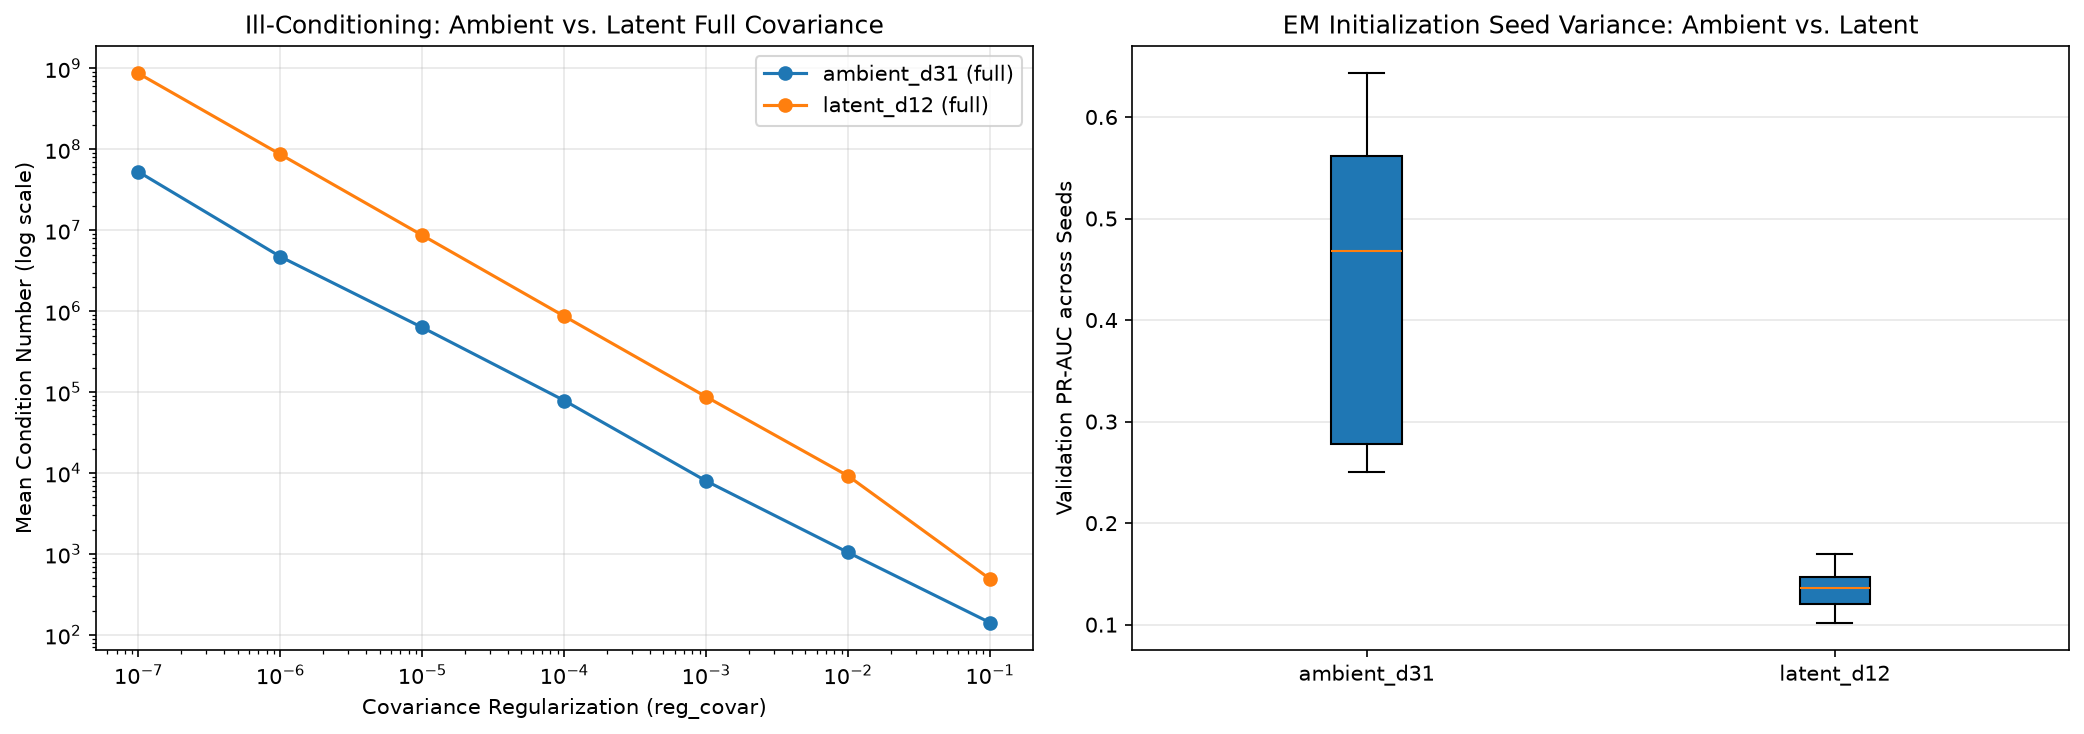
\includegraphics[width=\linewidth]{results/figures/latentgmm_stability_comparison.png}
\caption{Ambient ($d=31$) vs.\ latent ($d_z=12$) covariance condition-number sensitivity to $\varepsilon$ and multi-seed EM stability.}
\label{fig:latentgmm_stability}
\end{figure}

\paragraph{Latent Non-Gaussianity and Top-Rank Failure Mode.}
Marginal Shapiro--Wilk, skewness, and excess kurtosis audits on legitimate training coordinates explain why top-50 precision suffers ($0.00$ val, $0.02$ test at $K=50$) despite strong $0.5\%$~FPR recall. Whereas $38.71\%$ of $d=31$ ambient features are mildly Gaussian ($|\text{skew}| < 1$ and $|\text{kurtosis}| < 3$, mean $|\text{skew}| = 1.739$, mean Shapiro--Wilk $W = 0.8358$), \textbf{0.0\%} of the $12$ latent coordinates in \texttt{ae\_best.pt} satisfy mild Gaussianity: every latent axis is strongly right-skewed (mean $|\text{skew}| = 5.053$, median $3.778$, max $11.388$; mean $|\text{kurtosis}| = 84.639$; mean $W = 0.7135$). Because \texttt{UndercompleteAE} applies LeakyReLU at the bottleneck output, rare benign transactions pushed far along positive half-lines experience high quadratic Mahalanobis penalties under symmetric Gaussian components (maximum test NLL $246.35$), saturating the top-50 alert queue and suppressing PR-AUC relative to reconstruction error. Q--Q diagnostics confirm these heavy right tails (Fig.~\ref{fig:latentgmm_qq}). This aligns with Zong et~al.~\cite{zong2018deep} and Rezende and Mohamed~\cite{rezende2015variational}, who note that unconstrained deterministic bottlenecks need not be Gaussian-distributed.

\begin{figure}[!t]
\centering
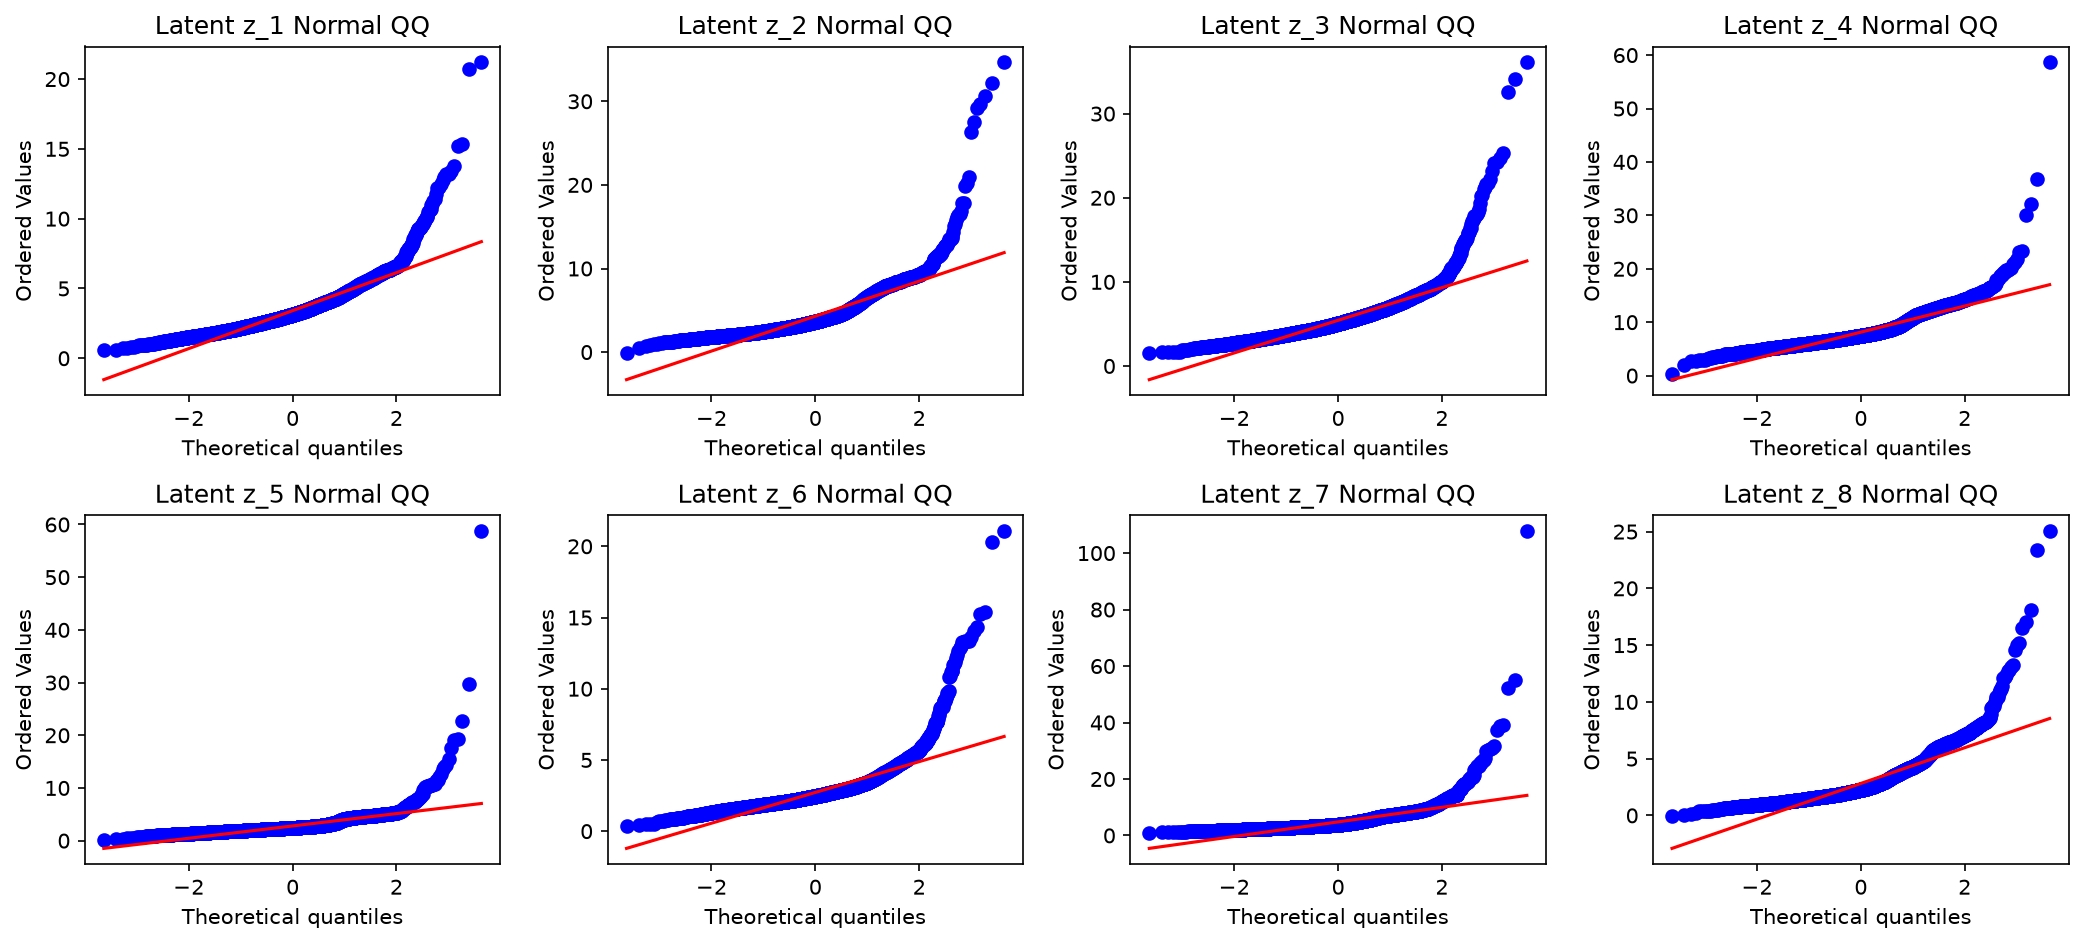
\includegraphics[width=\linewidth]{results/figures/latentgmm_qq_plots.png}
\caption{Normal Q--Q diagnostics for representative ambient vs.\ latent coordinates on legitimate training data, confirming severe right-skew induced by LeakyReLU bottleneck activations.}
\label{fig:latentgmm_qq}
\end{figure}

\paragraph{Complementarity with Parent Detectors.}
Despite lower overall PR-AUC, H1 captures fraud patterns missed by reconstruction error alone (Fig.~\ref{fig:latentgmm_2d}). At the $0.5\%$~FPR operating point on the test set ($75$ frauds), H1 catches $56$ frauds vs.\ $50$ for Phase~1 GMM ($47$ shared, $9$ H1-only, $3$ GMM-only; union recall $0.7867$) and vs.\ $51$ for its encoder parent AE ($48$ shared, $8$ H1-only, $3$ AE-only; union recall $0.7867$). On validation ($57$ frauds), H1 catches $40$ vs.\ $34$ for GMM ($9$ H1-only, union $0.7544$) and $38$ for AE ($4$ H1-only, union $0.7368$). Fraud transactions that lie within the linear subspace reconstructed well by AE can nonetheless sit at atypical coordinates within the latent manifold, making H1 a strong candidate for score-level fusion with reconstruction error.

\begin{figure}[!t]
\centering
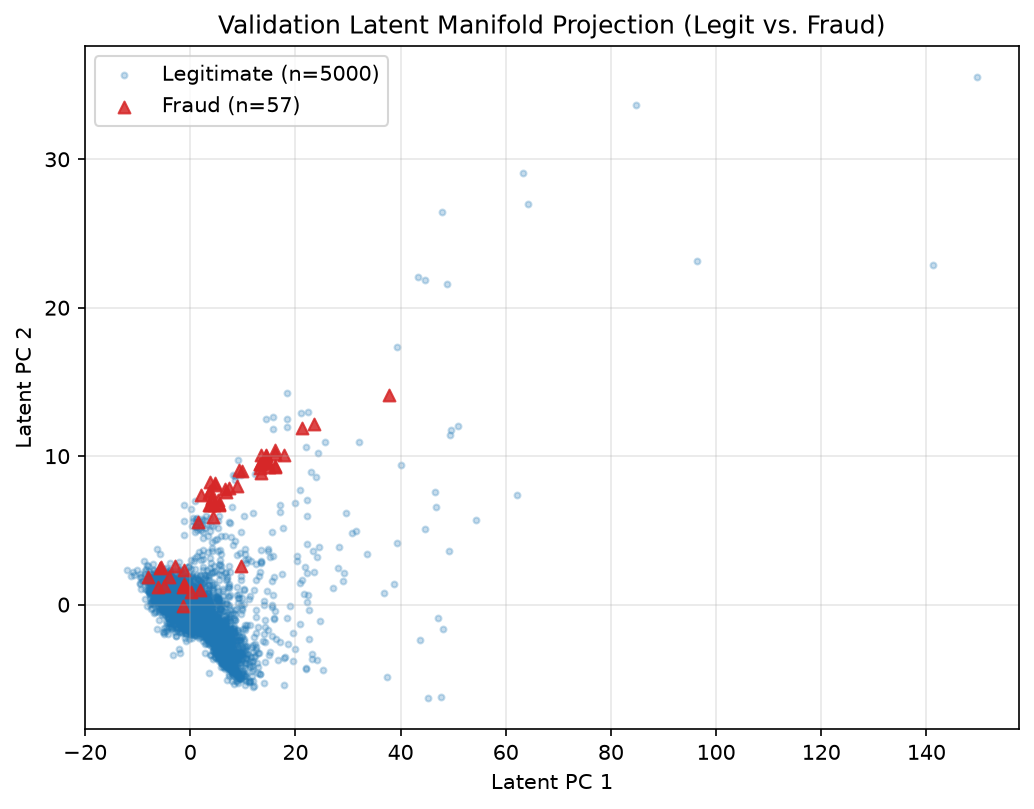
\includegraphics[width=\linewidth]{results/figures/latentgmm_2d_projection.png}
\caption{Two-dimensional latent projection of legitimate and fraudulent transactions with fitted latent-GMM density contours and false-positive/missed-fraud highlights.}
\label{fig:latentgmm_2d}
\end{figure}

\subsection{Latent Dimension Ablation Across Encoder Checkpoints}
\label{subsec:latentgmm_ablation}

Using Vani's latent-dimension ablation checkpoints ($k \in \{2, 4, 8, 16\}$) alongside \texttt{ae\_best.pt} ($k=12$), we evaluated $360$ GMM fits across four covariances, six component counts $K \in \{1, 2, 4, 8, 12, 16\}$, and three seeds ($\varepsilon = 10^{-4}$). Table~\ref{tab:ablation_gmm} and Fig.~\ref{fig:latentgmm_ablation_dim} summarize the best validation-PR-AUC GMM configuration for each bottleneck width.

\begin{table}[!t]
\centering
\caption{Best Latent-GMM Configuration per Bottleneck Dimension $k$ (Mean $\pm$ Std Across 3 Seeds, $\varepsilon = 10^{-4}$)}
\label{tab:ablation_gmm}
\begin{tabular}{lccccc}
\toprule
Bottleneck $k$ & Best Cov, $K$ & Params & Val PR-AUC & Test PR-AUC & Test Rec@0.5\% \\
\midrule
$k=2$  & full, 16  &  95 & $0.0053 \pm 0.0002$ & $0.0060 \pm 0.0004$ & 0.0133 \\
$k=4$  & full, 16  & 239 & $0.1674 \pm 0.0290$ & $0.2763 \pm 0.0627$ & 0.7644 \\
$k=4$  & tied, 16  &  89 & $0.1544 \pm 0.0227$ & $0.2920 \pm 0.0225$ & \textbf{0.7822} \\
$k=8$  & full, 16  & 719 & $0.0073 \pm 0.0006$ & $0.0113 \pm 0.0016$ & 0.0222 \\
$k=12$ (\texttt{ae\_best}) & tied, 16 & 285 & $0.1404 \pm 0.0251$ & $0.2443 \pm 0.0260$ & 0.7422 \\
$k=16$ & tied, 16  & 407 & \textbf{0.2637} $\pm$ 0.0391 & \textbf{0.4149} $\pm$ 0.0356 & 0.7733 \\
\bottomrule
\end{tabular}
\end{table}

\begin{figure}[!t]
\centering
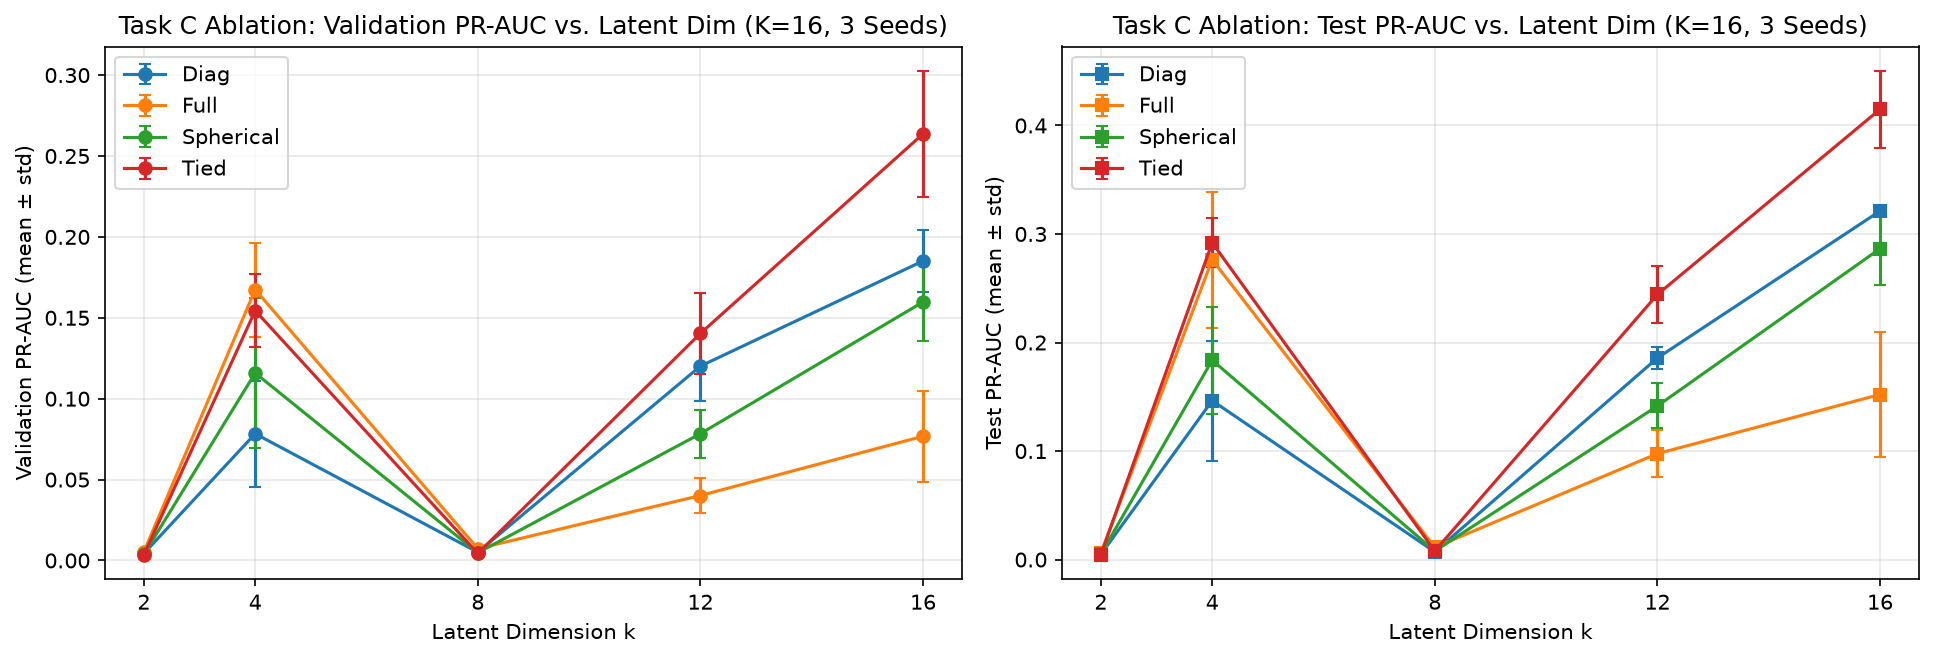
\includegraphics[width=\linewidth]{results/figures/latentgmm_ablation_dim.png}
\caption{Latent-GMM PR-AUC and Recall@0.5\%~FPR across Autoencoder bottleneck dimensions $k \in \{2, 4, 8, 12, 16\}$ and covariance structures.}
\label{fig:latentgmm_ablation_dim}
\end{figure}

Three findings emerge from this cross-checkpoint ablation. First, extreme compression ($k=2$) destroys class separation in latent space ($0.0060$ test PR-AUC). Second, bottleneck quality for \emph{density} modeling is non-monotonic with respect to reconstruction quality: at $k=8$, Vani's autoencoder achieves strong reconstruction PR-AUC ($0.2943$--$0.3017$ val in Table~\ref{tab:ae_reg} of Section~\ref{sec:p2_ae_results}), yet latent GMM drops to $0.0113$ test PR-AUC because the $k=8$ representation absorbs legitimate variance efficiently while pushing fraud deviation primarily into the reconstruction residual rather than distinct latent regions. Third, expanding capacity to $k=16$ with a regularized $\mathrm{tied}$ covariance ($K=16$, $407$ parameters) yields the strongest latent density detector ($0.2637$ val / $0.4149$ test PR-AUC and $0.7733$ test Recall@0.5\%~FPR), demonstrating that combining latent density with reconstruction residuals in a unified hybrid triage score (examined downstream) offers substantial headroom beyond standalone \texttt{ae\_best} ($k=12$).
